\subsection{Desktop Application}

The desktop application was designed with modularity and separation of concerns
in mind. There are three primary packages that make up the majority of the
system's functionality. These packages relate to the text file parser, the Ford-
Fulkerson algorithm and associated extensions, and the Swing user interface.
There are also separate packages for the league generation and the print/export
functionality. Each package can be considered to be a separate component of the
system.

This structure allows reimplementation or extension of individual components
without much modification of the other components. The structure also aided
development as there was a natural separation of tasks that could be assigned to
different team members.

Coupled to all other packages is the league package. This contains the
implementation of all common classes each component requires such as the
division, match, and team classes. This coupling was deemed to be required but
would still leave the application being well designed as coupling had been
mitigated or reduced between other components.

A diagrammatic representation of this organisation is shown in
Figure~\ref{fig:sysArch}

\begin{figure}
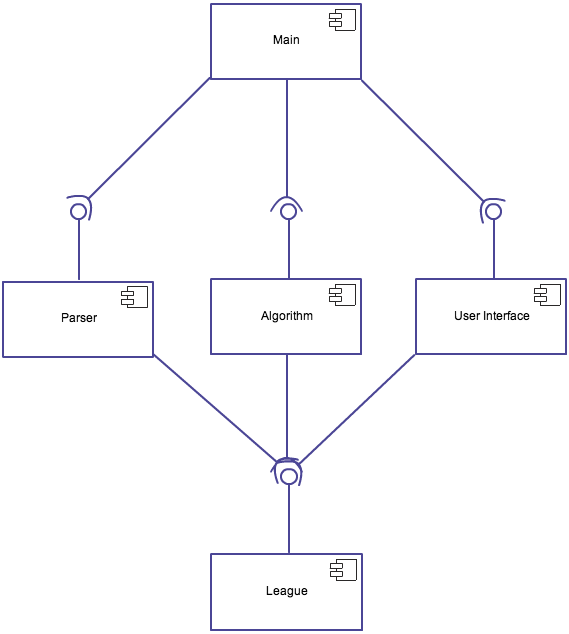
\includegraphics[width=\linewidth,keepaspectratio]
{images/DesktopApplicationSystemArchitecture.png}
\caption{System Architecture for Desktop Application}
\label{fig:sysArch}
\end{figure}
